\documentclass[../main]{subfiles}

\begin{document}

\setcounter{eqnarray}{0}
\setcounter{equation}{0}
\setcounter{figure}{0}

\clearpage

\part*{第2回}


\subsection{面積分}
\noindent
面積分の考え方に慣れる為に,以下の例を考える.\\
{\bf 例1}\\
\begin{figure}[htbp]
 \begin{center}
  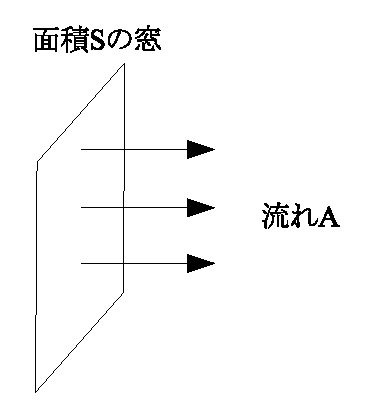
\includegraphics[width=50mm]{2.1.eps}
 \end{center}
 \caption{}
 \label{fig:one}
\end{figure}
\noindent
単位時間あたりの窓に垂直に入り込む風量を求めたい.単位時間単位面積あたりの風の流れを${\rm A[kgm^{-2}s^{-1}]}$とすると,求める量は${\rm AS[kgs^{-1}]}$である.\\
{\bf 例2}\\
次に窓が風の流れに垂直ではない場合を考える.
\begin{figure}[htbp]
 \begin{center}
  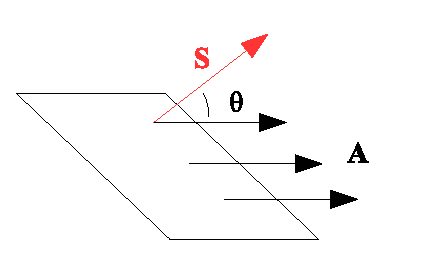
\includegraphics[width=50mm]{2.2.eps}
 \end{center}
 \caption{}
 \label{fig:one}
\end{figure}
風の流れをベクトル{\bf A}で表す.ここで面積を表すベクトル{\bf S}({\bf 面ベクトル})を,{\bf 向きが平面に垂直で,大きさが平面の面積に等しくなる}ようにとる.
面ベクトル{\bf S}と流れのベクトル{\bf A}のなす角を$\theta$とすると,単位時間に窓を垂直に通過する風量は
\begin{equation}
{\bf A}\cdot{\bf S}={\rm AS}\cos \theta
\end{equation}
このスカラー量を{\bf フラックス}\footnote{{\bf 流束}ともいいます.}(flux)という.\\

\noindent
{\bf 例3}\\
さて例1,2の話を一般化したい.そのために{\bf A}は物理量の流れを表すベクトル量とする.\\
任意の曲面で,位置ごとに流れが異なる曲面を考える.曲面を面積微小面$\bf \Delta S_i$(i=1,2,3...)に分割するとそれぞれの微小面での流れの方向は一定と考えることができ,微小部分でのフラックスは式(1)のように表すことができる.曲面全体にわたって微小部分のフラックスの和をとると
\begin{equation}
\sum_{i}^{}{\bf A_i}\cdot{\bf \Delta S_i}
\end{equation}
ここで$\bf \Delta S_i$を0に近づけ極限をとると,
\begin{equation}
\lim_{\bf \Delta S_i \rightarrow 0} \sum_{i}^{}{\bf A_i}\cdot{\bf \Delta S_i}= \int_{S}^{}{\bf A}({\bf r})\cdot{\bf dS}
\end{equation}
式(3)の右辺を,ベクトル場{\bf A}のSについての{\bf 面積分}という.\\

\noindent
{\bf 注1}: Sの各点で{\bf A}が法線方向(ただしその方向が,閉曲面の外から内か,内から外か,は閉曲面全体に渡って揃っているとする.)を向いており,大きさ$|{\bf A}|$=A が一定のとき.
\begin{equation}
\int_{S}^{}{\bf A}\cdot{\bf dS}=\int_{S}^{}|{\bf A}||{\bf dS}|\cos \theta=A \times \cos \theta \times \mbox{(閉曲面Sの面積)}
\end{equation}
\begin{equation}
\left \{
\begin{array}{l}
ベクトル場{\bf A}が閉曲面の内から外を向くとき\, \theta = 0\\
ベクトル場{\bf A}が閉曲面の外から内を向くとき\, \theta = \pi
\end{array}
\right.
\end{equation}

\noindent
{\bf 注2}: 面積分の結果は[{\bf A}の単位] $\times$ [面積の単位]の次元をもつ.

\subsection{Gaussの法則(積分形)}
内と外が定まった閉曲面をS,電場を{\bf E},S内の電荷をQ,真空の誘電率を$\varepsilon_0$とすると,以下の{\bf Gaussの法則}が成り立つ.
\begin{equation}
\varepsilon_0 \int_{S}^{} {\bf E} \cdot {\bf dS} = Q
\end{equation}
左辺をSを貫く{\bf 電束}(electrical flux)という.\\
式(6)から,Gaussの法則の意味は,{\bf 任意の閉曲面内の全電荷は,その閉曲面を貫く電束に等しい},ということだと分かる.\\
以下,{\bf Coulombの法則}と静電場の{\bf 重ね合わせの原理}によってGaussの法則を導出する.\\

\noindent
{\bf Step1}:1つの点電荷qを中心とする半径Rの球面Sの場合 \\
半径$R$の球の表面積は$4 \pi R^{2}$であり,点電荷が距離$R$離れた位置に作り出す電場の大きさは,第1回でやったように,$\frac{q}{4\pi \varepsilon_0 R^2}$であり,
この場合は式(4)が適応できるので,電気力線が球面を内側から外側に貫くことに注意すると
\begin{equation}
\varepsilon_0 \int_{S}^{} {\bf E} \cdot {\bf dS}=\varepsilon_0 \times E \times 4\pi R^2 = 4 \pi \varepsilon_0 R^2 \frac{q}{4\pi \varepsilon_0 R^2}=q
\end{equation}
となり,Gaussの法則(6)が成り立つ.\\

\noindent
{\bf Step2}:任意の閉曲面Sの内側に1つの点電荷がある場合 \\
まず補助定理から述べる.
\begin{figure}[htbp]
 \begin{center}
  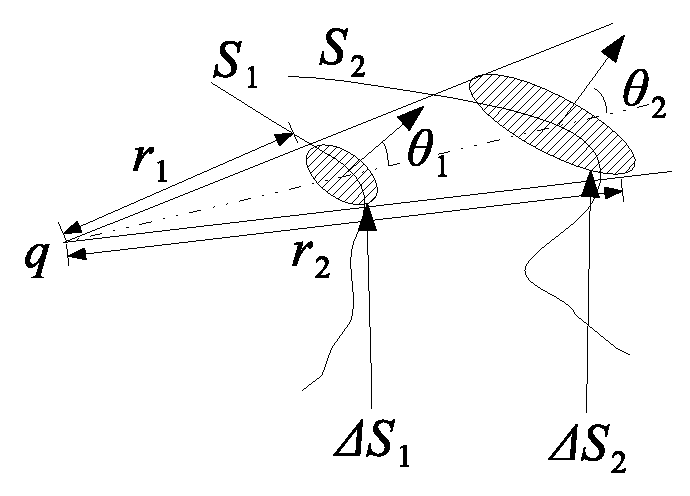
\includegraphics[width=60mm]{2.3.eps}
 \end{center}
 \caption{}
 \label{fig:one}
\end{figure}
図3の状況で以下の式が成立する.
\begin{equation}
\varepsilon_0 \int_{\Delta S_1}^{}{\bf E}{\bf dS} =\varepsilon_0 \int_{\Delta S_2}^{}{\bf E}{\bf dS}
\end{equation}
つまり微小面$\Delta S_1$と微小面$\Delta S_2$を貫く電気力線の本数が等しいということである.\\

\noindent
{\bf 証明} \\
(煩いので,両辺の$\varepsilon_0$は省略する.)\\
面ベクトル${\bf \Delta S_1}$と${\bf \Delta S_2}$と,それぞれの位置での電場のなす角をそれぞれ$\theta_1$ ,$\theta_2$とすると,
それぞれの面を貫く電束は,
\begin{eqnarray}
\int_{\Delta S_1}{}{\bf E}\cdot{\bf dS}=\frac{q}{4 \pi \varepsilon_0 {r_1}^2}\Delta S_1 \cos \theta_1 \\
\int_{\Delta S_2}{}{\bf E}\cdot{\bf dS}=\frac{q}{4 \pi \varepsilon_0 {r_2}^2}\Delta S_2 \cos \theta_2
\end{eqnarray}
ここで面ベクトルがそれぞれの位置における電場と垂直になるように面$\Delta S_1$と面$\Delta S_2$をそれぞれ$\theta_1$ ,$\theta_2$傾けると,その面積は$\Delta S_1 \cos \theta_1$,$\Delta S_2 \cos \theta_2$となる.傾けた二つの面は互いに平行となるから,傾けた面それぞれを底面,点電荷qのある点を頂点とする二つの錐体は相似な立体となる.したがって明らかに,
\begin{eqnarray}
\Delta S_1 \cos \theta_1 : \Delta S_2 \cos \theta_2 = {r_{1}}^2 : {r_{2}}^2 \Leftrightarrow \frac{\Delta S_1 \cos \theta_1}{{r_1}^2} = \frac{\Delta S_2 \cos \theta_2}{{r_2}^2}
\end{eqnarray}
これを式(9)あるいは式(10)に代入すると,ただちに,
\begin{eqnarray}
\int_{\Delta S_1}{}{\bf E}\cdot{\bf dS}=\int_{\Delta S_2}{}{\bf E}\cdot{\bf dS}
\end{eqnarray}
\begin{flushright}
(証明終)
\end{flushright}
さて$S_{1},S_{2}$は任意の閉曲面であるから,$S_{1}$を球面としても問題ない.すると式(7),(8)より,
\begin{eqnarray}
\varepsilon_0 \int_{S}{}{\bf E}\cdot{\bf dS}=\varepsilon_0 \int_{\mbox{球面}}{}{\bf E}\cdot{\bf dS}=q
\end{eqnarray}
したがって任意の閉曲面に対してもGaussの法則(6)が成り立つ.\\

\noindent
{\bf 注}: 閉曲面Sの外側に点電荷qがある場合は,式(8)の簡単な応用であり,\\
\begin{eqnarray}
\varepsilon_0 \int_{S}{}{\bf E}\cdot{\bf dS}=0
\end{eqnarray}

\noindent
{\bf Step3}:任意の静電場の場合 \\
空間の位置${\bf r}_i$に点電荷$q_i$が固定されているとする.(i=1,2,3,...)
点電荷$q_i$が位置{\bf r}につくる電場は,
\begin{eqnarray}
{\bf E}_i({\bf r}) = \frac{q_i}{4 \pi \varepsilon_0} \frac{{\bf r}-{\bf r}_i}{|{\bf r}-{\bf r}_i|^3}
\end{eqnarray}
電場には重ね合わせの原理が成り立つので,
\begin{eqnarray}
{\bf E}=\sum_{i}^{}{\bf E}_i
\end{eqnarray}
式(13),(16)より,
\begin{equation}
\varepsilon_0 \int_{S}{}{\bf E}\cdot{\bf dS}=\varepsilon_0 \int_{S}{}({\bf E}_1 + {\bf E}_2 + ...) \cdot {\bf dS} \\
=\varepsilon_0 \int_{S}{}{\bf E}_1 \cdot {\bf dS} + \varepsilon_0 \int_{S}{}{\bf E}_2 \cdot {\bf dS} + ... \\
= \sum_{i}^{} q_i = Q
\end{equation}
したがって,任意の静電場にGaussの法則(6)が成り立つ.

\subsection{Gaussの法則の応用}
\noindent
{\bf 半径rの球面Sの中心に点電荷qが存在する場合} \\
点電荷から出る全ての電気力線は,点電荷を中心とする球面と直交するので,式(4),(6)から
\begin{equation}
\varepsilon_0 \times 4 \pi r^2 \times E_r = q \Leftrightarrow E_r = \frac{q}{4 \pi \varepsilon_0 r^2}
\end{equation}
これで,Gaussの法則からCoulombの法則を導くことができた.\\

\noindent
{\bf 半径rの球内一様に電荷が分布している場合}\\
$ 0 \leq r \leq a $の場合\\
\begin{equation}
\varepsilon_0 \times 4 \pi r^2 \times E_r = Q {\left(\frac{r}{a} \right)}^3 \Leftrightarrow E_r = \frac{Q}{4 \pi \varepsilon_0 a^3}r
\end{equation}
$a \leq r$の場合\\
\begin{equation}
\varepsilon_0 \times 4 \pi r^2 \times E_r = Q \Leftrightarrow E_r = \frac{Q}{4 \pi \varepsilon_0 r^2}
\end{equation}

\begin{figure}[htbp]
 \begin{center}
  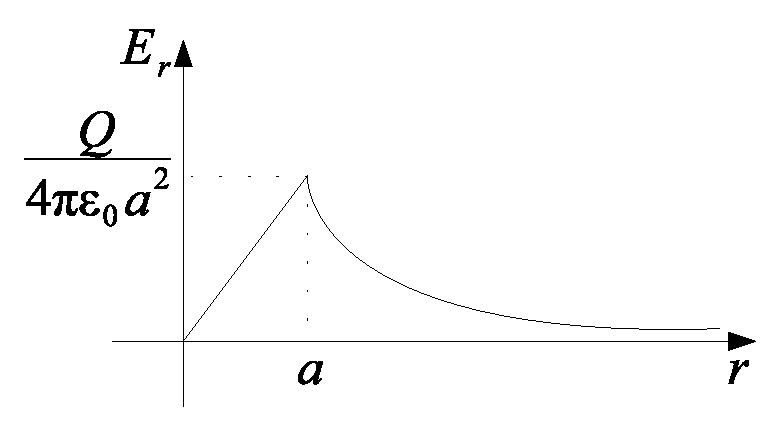
\includegraphics[width=50mm]{2.4.eps}
 \end{center}
 \caption{}
 \label{fig:one}
\end{figure}

\end{document}
